\subsection{Introduction}
	This section is divided in two parts, the first one describe the implementation of the algorithm in a laptop computer. The objective is to get a reference to compare the results of the final implementation. The second one is a description of the final application and its results.
	During this experiments, five datasets were used. These datasets were provided by the GRVC, captured in the testbed of CATEC \cite{CATEC}, and were used previously by a partner. These datasets, composed by a number of images and data provided by a VICON system (Time, position and orientation of quadrotors), and Representing different situations, yielded a number of interesting results that will be gathered at the end of this chapter. 

	\begin{figure}[h]
		\centering
		\begin{subfigure}{0.49\linewidth}
			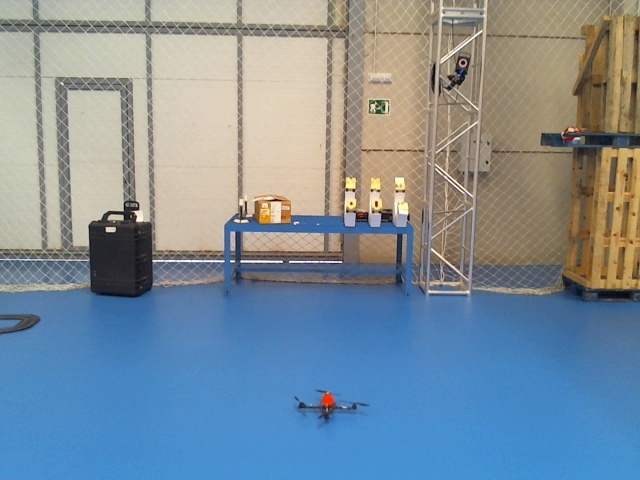
\includegraphics[width=\linewidth]{../Images/c4/image_ori}
			\caption{Original Image}
			\label{fig:image_ori}
		\end{subfigure}
		%--------------------------------------------------------------------
		\begin{subfigure}{0.49\linewidth}
			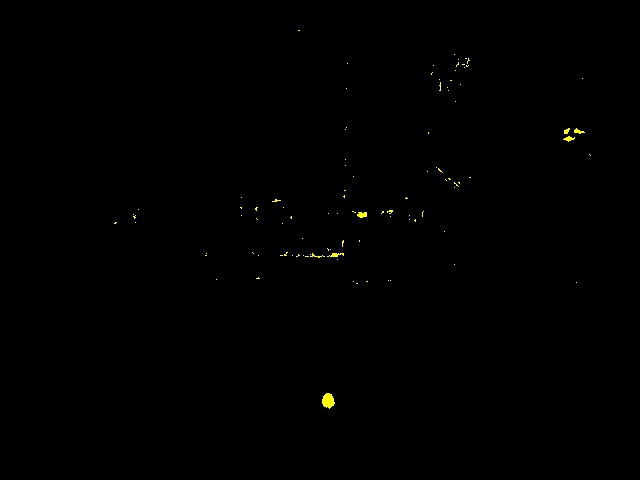
\includegraphics[width=\linewidth]{../Images/c4/image_seg}
			\caption{Segmented Image}
			\label{fig:image_seg}
		\end{subfigure}
		\caption{Images to and from algorithm}
		\label{fig:frames_PC}
	\end{figure}

	Figure: \ref{fig:frames_PC} shows an example of captured image from the camera and the result of the segmentation algorithm. Particularly, we were looking for orange color (The cap of the quadrotor in this case). However unlike simulation, where there was only one object as the result of segmentation, the algorithm return many targets. The first sift is by size, we do not consider tiny objects that use to be noise and are quantitative smaller than the target.
		
	
	Following sections shows the results of the described algorithm while running completely on the same computer and afterwards using the definitely structure of the system (Ground Station on PC and the capture and segmentation on the onboard computer) with the provided datasets.

\subsection{Complete Test in PC}
	PC's and other's characteristics:
	\begin{itemize}
		\item{Pictures of 640x480}
		\item{Intel core i7 2.20 GHz. Usage 7-10\%}
		\item{6 GB of RAM. Usage $\sim$ 5000-7000 KB}
	\end{itemize}
	\subsubsection{Ground Tracking algorithm}
	
	All datasets have information about two cameras tracking a target. However, in this experiment, we use only the information about the first  of the camera. The following table shows the medium time and speed of every step of the algorithm: \\
	
	{
	\centering
		\begin{tabular}{|c|c|c|c|c||c|}
		\hline  					&  Open Image	&  RGB to HSV 	& Segmentation 	& EKF step  & Complete \\ 
		\hline  \textbf{time (ms)}	& 0.0085 		& 0.0015 		& 0.0100 		& 0.0001 	& 0.0231 	\\ 
		\hline  \textbf{fps (1/s)}	&  118			&  645			&  100			& 13936 	& 43 		\\ 
		\hline 
		\end{tabular} 
	}
	\newline

	{
	\label{Reference_fps_table}
	This application runs sequentially, so the "complete"\footnote{The complete time has a higher value, than the addition of the previous, because it includes some GUI process} time of the process is the addition of the previous ones. Therefore, It is possible to reduce the complete process time using multi-threading (or in other words increase the FPS). In the following section will be described the results of the process with multi-threading inside the onboard computer. \ref{test_with_odroid_and_GT}
	}
	
	The next graphs shows the original and estimated position of the target \ref{fig:trajectories_PC} and the error between both \ref{fig:errors_PC}. In general terms, the errors associated with each axis are bounded below 0.2 m.
	
	\begin{figure}[hp]
		\centering
		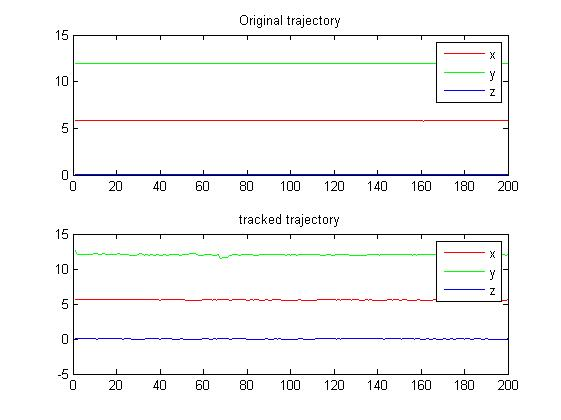
\includegraphics[width=0.75\linewidth]{../Images/c4/trajs}
		\caption{Original and tracked trajectories}
		\label{fig:trajectories_PC}
	\end{figure}
	
	\begin{figure}[hp]
		\centering
		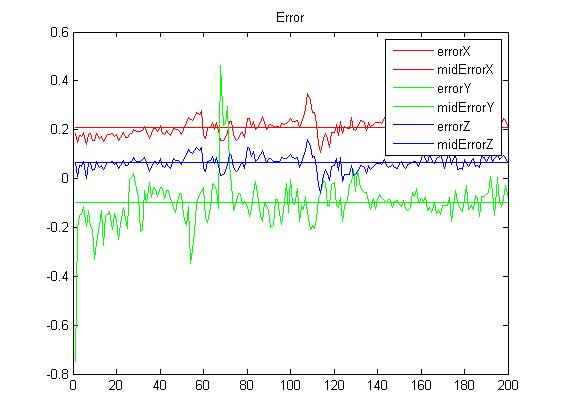
\includegraphics[width=0.5\linewidth]{../Images/c4/errors}
		\caption{Error between real and tracked trajectories}
		\label{fig:errors_PC}
	\end{figure}
	
	\newpage
	
	%\begin{figure}[ht]
	%	\centering
	%	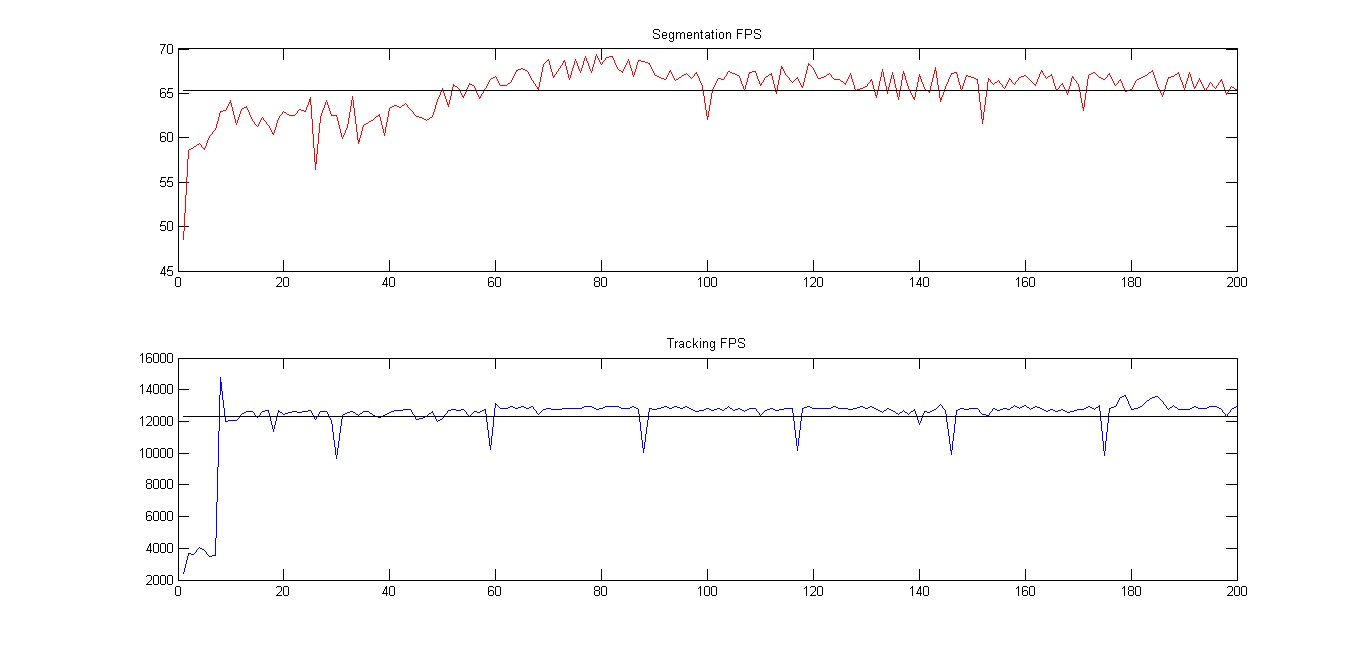
\includegraphics[width=\linewidth]{../Images/c4/fps}
	%	\caption{}
	%	\label{fig:fps_PC}
	%\end{figure}
		
	\subsubsection{Stereo Tracking algorithm}
	
	On this case, we use the data about both of the cameras. As previously, the following table collect time information about the process of the application. \\
		
	{                
	\centering
		\begin{tabular}{|c|c|c|c|c||c|}
		\hline  					&  Open Image	&  RGB to HSV 	& Segmentation 	& EKF step  & Complete \\ 
		\hline  \textbf{time (ms)}	&	0.0222		& 	0.0031 		&  	0.0157		&  	0.0001 	&  0.0429		\\ 
		\hline  \textbf{fps (1/s)}	& 	45 			& 	321.5 		& 	63.8 		& 7672.5	&  23.3		\\ 
		\hline 
		\end{tabular} 
	}
	\newline
	
	This table has the same annotation that the previous one \ref{Reference_fps_table}.
	
	Eventually, these figures shows the position of the target, the result of the estimation \ref{fig:trajectories_stereo_PC} and the error between both \ref{fig:errors_stereo_PC}.
	
	\begin{figure}[hp]
		\centering
		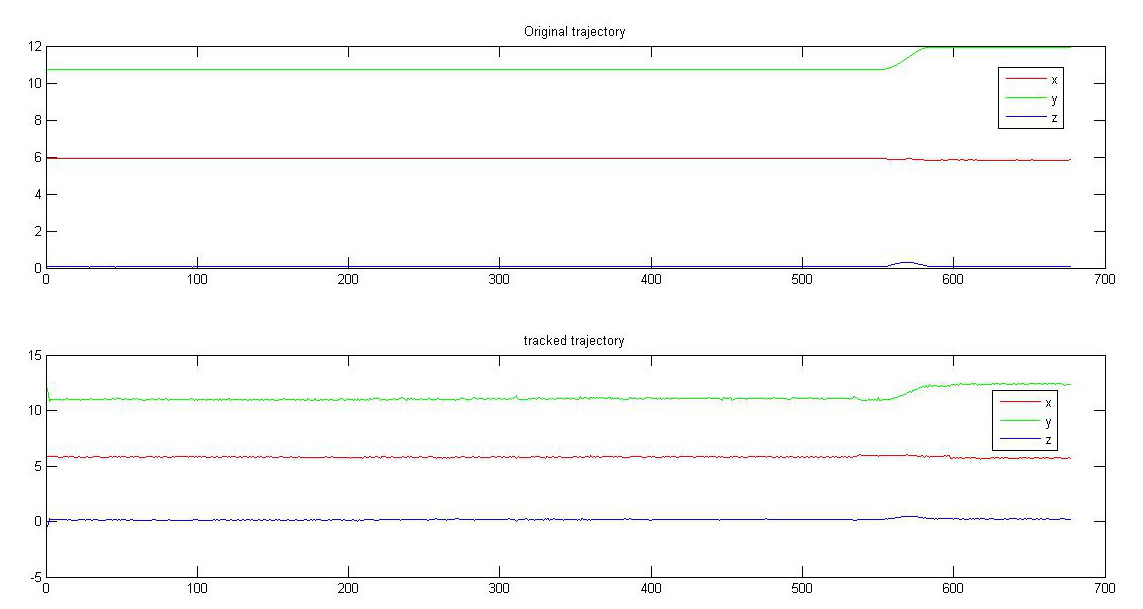
\includegraphics[width=\linewidth]{../Images/c4/trajs_stereo}
		\caption{Original and tracked trajectories}
		\label{fig:trajectories_stereo_PC}
	\end{figure}
	
	\begin{figure}[htp]
		\centering
		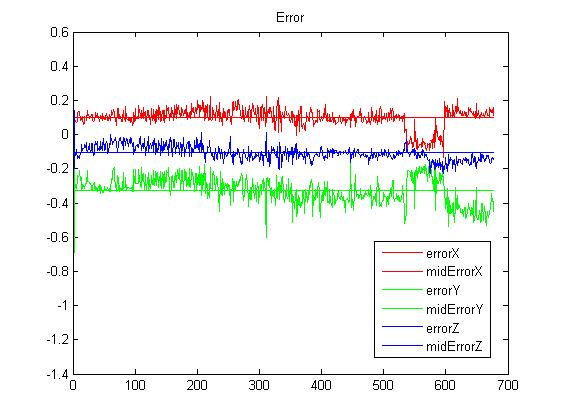
\includegraphics[width=0.7\linewidth]{../Images/c4/errors_stereo}
		\caption{Error between real and tracked trajectories}
		\label{fig:errors_stereo_PC}
	\end{figure}	
	
	\newpage
	
\subsection{Test with Odroid and Ground Station}
	\label{test_with_odroid_and_GT}

	\subsubsection{Ground Tracking algorithm}
	
	\subsubsection{Stereo Tracking algorithm}